\documentclass{beamer}
\usepackage{graphicx} % Required for inserting images
\usepackage{undertilde}
\usepackage{subcaption}
\newcommand{\Phit}{\tilde{\Phi}}
\newcommand{\rhot}{\tilde{\rho}}
\newcommand{\R}{\mathbb{R}}
\newcommand{\n}{\mathbf{n}}
\newcommand{\ei}{\epsilon_\infty}
\newcommand{\es}{\epsilon_s}
\newcommand{\ep}{\epsilon_p}
\newcommand{\emem}{\epsilon_m}
\newcommand{\ez}{\epsilon_0}
\newcommand{\ph}{\Phi}
\newcommand{\ps}{\Psi}
\newcommand{\EE}{\mathbf{E}}
\newcommand{\xx}{{\mathbf a}}
\newcommand{\ee}{{\mathbf e}}
\newcommand{\pp}{{\mathbf p}}
\newcommand{\dd}{{\mathbf d}}
\newcommand{\rr}{{\mathbf r}}
\newcommand{\s}{{\mathbf s}}
\newcommand{\cg}{{\cal M}} %base finite element space; conjugate galerkin, or lagrange
\newcommand{\test}{{\cal M}_0} %so-called 'test' function space; elements in cg which vanish on dirichlet boundaries
\newcommand{\nn}{{\mathbf n}}
\title{Nonlocal Size Modified Ion Channel Models and Fast Finite Element Solvers }
\author{Liam Jemison }
\date{August 2024}

\begin{document}
\begin{frame}
    \titlepage
\end{frame}
\section{Introduction}
\begin{frame}{Outline}
    \tableofcontents
\end{frame}
\begin{frame}{Ion Channels}
    Ion channels are a type of protein, found abundantly in living organisms. We are particularly interested in studying Voltage-Dependent Anion Channels (VDACs), a class of large pores found in the outer mitochondrial membrane (OMM) of humans and animals. 
\end{frame}
\begin{frame}{Domain Geometry}
We consider a box region $\Omega$ containing three distinct physical regions:
\begin{itemize}
    \item The protein region $D_p$ containing a VDAC protein, consisting of $n_p$ atoms, with charges $z_1, \ldots z_{n_p}$;
    \item The membrane region $D_m$ containing a portion of the OMM;
    \item The solvent region $D_s,$ which is filled with water, and $n$ species of ions or metabolites, carrying charges $Z_1, \ldots , Z_n.$ 
\end{itemize}
\end{frame}
\begin{frame}{Domain Geometry}
\centering
\begin{figure}
    \centering
        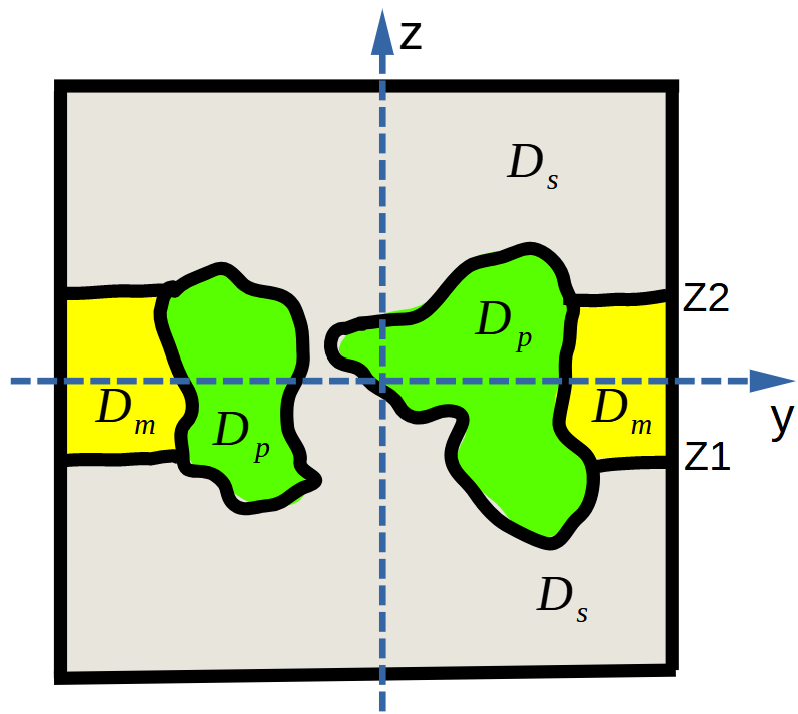
\includegraphics[width=0.4\textwidth]{figures/domain.png}
    \caption{A cross section of $\Omega$ along $x = 0.$}
\end{figure}

\end{frame}

\begin{frame}{Nonlocal Poisson Boltzmann Ion Channel Model}
    The major work of this thesis is to propose a modified Poisson-Boltzmann model describing VDACs in solution, that includes nonlocal terms arising from the structure of the surrounding solvent, and to implement efficient finite element solvers to solve this nonlocal Poisson-Boltzmann Ion Channel model. 

    This is an extension of previous work that uses a local Poisson-Boltzmann approach to describe the electrostatics of VDAC in solution. 
\end{frame}
\section{Electrostatics}
\begin{frame}{Electrostatics}
The electric field $\ee$ produced by a charge distribution $\rho$ satisfies, according to Gauss's law, 
    \begin{align}\label{eq:gauss}
        \ez \nabla \cdot \ee = \rho,
    \end{align}
where $\ez$ is a physical constant. When the charge sources are assumed to be stationary, the field $\ee$ can be expressed as the gradient of a scalar function:
\begin{align}\label{eq:irrotational}
    \ee = -\nabla \Phi.
\end{align}
The scalar function $\Phi$ is called the (electrostatic) potential function. 
\end{frame}
\begin{frame}{Electrostatics}
    The components of the biological system we are interested in -- a VDAC embedded in the OMM, in solution -- are insulating, or dielectric, materials, that is, materials which do not contain free electrons (in contrast to a conductor, such as a metal).  
\end{frame}

\begin{frame}{Dielectrics}
    Placing a dielectric material into water causes a realignment of the atomic structure of the water molecules. The water molecules form dipoles, an action called polarization, which produces a field, which interacts with the field produced by the dielectric material, which is called the displacement field. There are thus two sources of of charge density: one due to free charges ($\rho$), and another due to polarization ($\gamma$). We write 
    \begin{align}\label{eq:gauss-dielectric}
        \ez \nabla \cdot \ee = \rho + \gamma. 
    \end{align}
\end{frame}
\begin{frame}{Linear Dielectrics}
    It is common to assume that the displacement field is proportional to the total electric field. For us, this looks like 
    \begin{align}
            \dd(\rr) &= \begin{cases}
		\ez \ep \ee(\rr), & \rr \in D_p, \\
		\ez \emem\ee (\rr), & \rr \in D_m, \\
		\ez \es \ee(\rr) , & \rr \in D_s.
	\end{cases} \label{eq:linear-dielectric}
    \end{align}
    The constants $\es, \ep, \emem$ are permittivity constants associated with the physical regions $D_s, D_p, D_m.$
\end{frame}
\begin{frame}{Nonlocal Dielectrics}
    We are interested in replacing the linear dielectric relationship \eqref{eq:linear-dielectric} with 

    \begin{align}
    \dd(\rr) &= \begin{cases}
		\ez \ep \ee(\rr), & \rr \in D_p, \\
		\ez \emem\ee (\rr), & \rr \in D_m, \\
		\ez \ei \ee(\rr) + \ez(\es - \ei) \int_{D_s} e(\rr') Q_\lambda(\rr - \rr') d\rr', & \rr \in D_s.
	\end{cases} \label{eq:dielectric}
\end{align}
Where $Q_\lambda$ is a kernel function, introduced to incorporate charge correlations in the ionic solution in $D_s.$
\end{frame}
\begin{frame}{Nonlocal Kernel}
    Here, we take the kernel function $Q_\lambda$ to be
    \begin{align}\label{eq:qlam}
        Q_{\lambda}(\rr)=\frac{e^{-|\rr|/\lambda}}{4\pi \lambda^2 |\rr|},
    \end{align}
    where $\lambda$ is a parameter, referred to as the correlation or screening length.  The selection \eqref{eq:qlam} has a number of desirable properties: it is isotropic, satisfies causality principles, a notion of themodynamic stability, limits to the local Poisson equation as $\lambda \to 0,$ and, usefully, is the Green's function for a particular linear PDE. Indeed, we have 
    \begin{align}\label{eq:qlam-fts}
        -\lambda^2 \Delta Q_\lambda(\rr) + Q_\lambda(\rr) = \delta (\rr), \qquad \rr \in \mathbb{R}^3.
    \end{align}
\end{frame}
\begin{frame}{Free Charge Sources}
    We assume that the charge density is due to charges from the concentration functions in $D_s$ and point charges in the protein region, or that 

\begin{align}
    \rho(\rr) &= \begin{cases}
        e_c \sum_{j=1}^{n_p} z_j \delta_{\rr_j}(\rr), &\rr \in { D_p}, \\
	   e_c \sum_{i=1}^n Z_i c_i(\rr), &\rr \in { D_s}, \\
	    0, &\rr \in { D_m}. 
    \end{cases} \label{eq:free-charge}
\end{align}
\end{frame}
\section{Nonlocal Dielectric Poisson Model}
\begin{frame}{Nonlocal Poisson Equations}
    Substituting the free charge distribution \eqref{eq:free-charge} and the electrostatic assumption \eqref{eq:irrotational} into the nonlocal dielectric relationship \eqref{eq:dielectric}, one obtains Poisson equations for the electrostatic potential $\Phi:$

    \begin{align}
    -\epsilon_p\Delta\Phi(\rr) &= \frac{e_{c}}{\epsilon_0}\sum\limits_{j=1}^{n_{p}}z_{j} \delta_{\rr_{j}}, & \rr \in D_p,\\
-\epsilon_{\infty}\Delta\Phi(\rr) - (\epsilon_s-\epsilon_{\infty}) \Delta(\Phi\ast  Q_{\lambda})(\rr)
&= \frac{e_{c}}{\epsilon_0}\sum\limits_{i=1}^{n}Z_{i}c_{i}(\rr), & \rr \in D_s,\\
-\epsilon_m \Delta \Phi(\rr) &= 0, & \rr \in D_m. 
\end{align}
\end{frame}

\begin{frame}{Nonlocal Dielectric Poisson Model}
    We fill out boundary conditions by assuming that the potential $\Phi$ and displacement field $\dd$ are continuous in the normal direction, along each sub-region interface, and we take a Dirichlet condition on the top and bottom of $\Omega,$ which we will denote $\Gamma_D,$ and a Neumann condition on the sides of $\Omega,$ which we will denote $\Gamma_N.$
\end{frame}
\begin{frame}{Nonlocal Dielectric Poisson Model}
    We summarize:
    \begin{align}
\label{phi-u1}
  \left\{\begin{array}{cl}
    -\epsilon_p\Delta\Phi(\rr) = \frac{e_{c}}{\epsilon_0}\sum\limits_{j=1}^{n_{p}}z_{j} \delta_{\rr_{j}}, & \rr \in D_p,\\
-\epsilon_{\infty}\Delta\Phi(\rr) - (\epsilon_s-\epsilon_{\infty}) \Delta(\Phi\ast  Q_{\lambda})(\rr) 
= \frac{e_{c}}{\epsilon_0}\sum\limits_{i=1}^{n}Z_{i}c_{i}(\rr), & \rr \in D_s,\\
-\epsilon_m \Delta \Phi(\rr) = 0, & \rr \in D_m, \\
\Phi(\s^{-}) = \Phi(\s^{+}), & \s\in\Gamma_p,\\
\epsilon_p\frac{\partial\Phi(\s^{-})}{\partial \nn_p(\s)} = \epsilon_\infty\frac{\partial\Phi(\s^{+})}{\partial \nn_p(\s)}+(\epsilon_s-\epsilon_\infty)\frac{\partial (\Phi\ast Q_{\lambda})(\s)}{\partial \nn_p(\s)}, & \s\in\Gamma_p,\\[0.2em]
\Phi(\s^{-}) = \Phi(\s^{+}), & \s\in\Gamma_m,\\
\epsilon_m\frac{\partial\Phi(\s^{-})}{\partial \nn_m(\s)} = \epsilon_\infty\frac{\partial\Phi(\s^{+})}{\partial \nn_m(\s)}+(\epsilon_s-\epsilon_\infty)\frac{\partial (\Phi\ast Q_{\lambda})(\s)}{\partial \nn_m(\s)} + \tau \sigma, & \s\in\Gamma_m,\\[0.2em]
\Phi(\s^{-}) = \Phi(\s^{+}), \quad  \epsilon_p\frac{\partial\Phi(\s^{-})}{\partial \nn_p(\s)} = \epsilon_m\frac{\partial\Phi(\s^{+})}{\partial \nn_p(\s)}, \quad &\s \in \Gamma_{pm}, \\
   \Phi(\s) = \bar{g}(\s), & \s \in \Gamma_D, \\
   \frac{\partial \Phi(\s)}{\partial \nn_b(\s)} = 0, & \s \in \Gamma_N.
  \end{array}
\right
.
\end{align}
\end{frame}

\begin{frame}{Dimensionless Potential}
    We customarily express the model in terms of a dimensionless potential $u.$ 
    \begin{equation}
\label{nonlocal-Poisson-u}
 \left\{\begin{array}{cl}
     -\epsilon_p\Delta u(\rr) =\alpha \sum\limits_{j=1}^{n_{p}}z_{j}  \delta_{\rr_{j}}, & \rr \in D_p,\\
-\epsilon_{\infty}\Delta u - (\epsilon_s-\epsilon_{\infty}) \Delta(u\ast  Q_{\lambda})(\rr)
= \beta \sum\limits_{i=1}^{n}Z_{i}c_i(\rr), & \rr \in D_s,\\
-\epsilon_m \Delta u(\rr) = 0, & \rr \in D_m \\
u(\s^{-}) = u(\s^{+}), & s \in \Gamma_p\\
\epsilon_p\frac{\partial u(\s^{-})}{\partial \nn_p(\s)} = \epsilon_\infty\frac{\partial u(\s^{+})}{\partial \nn_p(\s)}+(\epsilon_s-\epsilon_\infty)\frac{\partial (u\ast Q_{\lambda})(\s)}{\partial \nn_p(\s)}, & \s\in\Gamma_p,\\
u(\s^{-}) = u(\s^{+}), s \in \Gamma_m\\
\epsilon_m\frac{\partial u(\s^{-})}{\partial \nn_m(\s)} = \epsilon_\infty\frac{\partial u(\s^{+})}{\partial \nn_m(\s)}+(\epsilon_s-\epsilon_\infty)\frac{\partial (u\ast Q_{\lambda})(\s)}{\partial \nn_m(\s)} + \tau \sigma, & \s\in\Gamma_m,\\
u(\s^{-}) = u(\s^{+}), \quad  \epsilon_p\frac{\partial u(\s^{-})}{\partial \nn_p(\s)} = \epsilon_m\frac{\partial u(\s^{+})}{\partial \nn_p(\s)}, \quad &\s \in \Gamma_{pm} \\
   u(\s) = g(\s), & \s \in \partial \Omega, \\
   \frac{\partial u (\s)}{\partial \nn_b(\s)} = 0, & \s \in \Gamma_N
\end{array}
\right.
\end{equation}  
\end{frame}
\begin{frame}{Concentration functions}
    In the classic Poisson-Boltzmann theory, the concentration functions are assumed to satisfy a Boltzmann distribution:
    \begin{align}
    c_i(\rr) = c_i^b e^{-Z_i u(\rr)}, \qquad i = 1,\ldots , n,
\end{align}
where $c_i^b$ denotes the bulk concentration of the $i$th ionic species. This choice can be motivated as the minimizer of a particular electrostatic free-energy functional. 
\end{frame}
\begin{frame}{Size modifications}
    A slightly more sophisticated approach is to select the concentration functions to minimize a modified energy functional which incorporates steric effects,
    % \footnote{Originally due to Andelman, Borukhov, Orland 1997 \emph{steric effects in electrolytes}, expounded on by Li 2009 and then a series of papers by Xie }, l
    leading to 
    \begin{equation}
 \label{c-selection}
  c_i(\rr) = \frac{c_i^b e^{-Z_{i} u(\rr)} }{1 +  \gamma  v   \sum\limits_{j=1}^n c_j^b e^{-Z_{i} u(\rr)} }, \quad \rr \in D_s, \quad i=1,2,\ldots, n,
\end{equation}
in the case of ions with uniform size $v$ or the nonlinear system 
\begin{equation}\label{size-constraints}
 c_{i}(\rr) - {c}_{i}^b  \left[1-  \gamma  \sum\limits_{j=1}^n  v_j c_j(\rr)  \right]^{\frac{ v_i}{v_0}} e^{-Z_{i} u(\rr)} =0,
\end{equation}
for $r \in D_s$ and $i = 1, \ldots n,$ when the ionic species have nonuniform sizes $v_1,\ldots, v_n.$
\end{frame}
\begin{frame}{Solving nonlocal PB equations for Ion Channels}
    We present a solution decomposition approach to solving the nonlocal model \eqref{nonlocal-Poisson-u}. This approaches solves a series of sub-problems and then reconstructs $u$ as the sum
    \begin{align}
        u = G + \Psi + \Phit.
    \end{align}
\end{frame}
\begin{frame}{Solving nonlocal PB equations for Ion Channels}
    Here $G$ is the analytical solution to 
    \begin{align}
            \begin{cases}
            -\epsilon_p \Delta G(\rr) = \alpha \sum\limits_{j=1}^{n_{p}}z_{j}  \delta_{\rr_{j}}, \qquad \rr \in \mathbb{R}^3,
        \end{cases}
    \end{align}
    given by 
    \begin{align}
        G(\rr) = \frac{\alpha}{4\pi\ep}  \sum\limits_{j=1}^{n_p}\frac{z_{j}}{| \rr-\rr_j |}. 
    \end{align}
\end{frame}
\section{Solution Decomposition}
\begin{frame}{Solving nonlocal PB equations for Ion Channels}
   The function $ \Psi$ is the solution of the linear nonlocal interface problem
 \begin{equation}\label{eq:psi}
\left\{
\begin{array}{cl}
\Delta\Psi(\rr) = 0, & \rr \in D_p, \\
\Delta\Psi(\rr) = 0, & \rr \in D_m, \\
-\epsilon_\infty\Delta\Psi(\rr) -  (\epsilon_s-\epsilon_\infty)\Delta (\Psi \ast Q_{\lambda})=  (\epsilon_s-\epsilon_\infty)\Delta(G\ast Q_{\lambda}), & \rr \in D_s,\\
\Psi(\s^{-}) =\Psi(\s^{+})  &  \s\in\Gamma_p, \\
  \epsilon_p\frac{\partial\Psi(\s^{-})}{\partial \nn_p(\s)} -  \epsilon_{\infty}\frac{\partial\Psi(\s^{+})}{\partial \nn_p(\s)} 
 =  (\epsilon_s-\epsilon_\infty)\frac{\partial (\Psi \ast Q_{\lambda})(\s)}{\partial \nn_p(\s)} +g_{\Gamma_p}(\s), &  \s\in\Gamma_p,\\
 \Psi(\s^{-}) =\Psi(\s^{+}), &\s\in\Gamma_m, \\  
  \epsilon_m\frac{\partial\Psi(\s^{-})}{\partial \nn_m(\s)} -  \epsilon_{\infty}\frac{\partial\Psi(\s^{+})}{\partial \nn_m(\s)} 
 =  (\epsilon_s-\epsilon_\infty)\frac{\partial (\Psi \ast Q_{\lambda})(\s)}{\partial \nn_m(\s)} +g_{\Gamma_m}(\s), &  \s\in\Gamma_m,\\
 
\epsilon_p \frac{\partial \Psi (\s^{-})}{\partial \nn_p(\s)} - \epsilon_{m}\frac{\partial \Psi (\s^{+})}{\partial \nn_p(\s)} = (\epsilon_m - \epsilon_p) \frac{\partial G}{\partial \nn_p} (\s), & \s \in \Gamma_{pm} \\
\Psi(\s) = g(\s) - G(\s), & \s \in \Gamma_D, \\
\frac{\partial \Psi (\s)}{\partial \nn_b(\s)} = \frac{\partial G(\s)}{\partial \nn_b(\s)}, & \s \in \Gamma_N.
\end{array}
\right.
\end{equation}
\end{frame}

\begin{frame}{Solving nonlocal PB equations for Ion Channels}
    Here  $g_{\Gamma_p}, g_{\Gamma_m}$ are defined by
\begin{align}
\label{g-def}
g_{\Gamma_p}(\s) &=  (\epsilon_s-\epsilon_\infty)\frac{\partial (G\ast Q_{\lambda})(\s)}{\partial \nn(\s)} + (\epsilon_\infty-\epsilon_p)\frac{\partial G(\s)}{\partial \nn(\s)}, \\
g_{\Gamma_m}(\s) &=  (\epsilon_s-\epsilon_\infty)\frac{\partial (G\ast Q_{\lambda})(\s)}{\partial \nn(\s)} + (\epsilon_\infty-\epsilon_m)\frac{\partial G(\s)}{\partial \nn(\s)}.
\end{align}
\end{frame}
\begin{frame}{Solving nonlocal PB equations for Ion Channels}
    And finally $ \Phit$ is a solution of the nonlinear nonlocal interface problem:
    \begin{equation}\label{eq:phit}
    \left\{
    \begin{array}{cl}
    \Delta \Phit (\rr) = 0, & \rr\in D_p \cup D_m,\\
    -\epsilon_\infty\Delta \Phit  - (\epsilon_s-\epsilon_\infty)\Delta(\Phit \ast Q_{\lambda}) =
    \beta \sum\limits_{i=1}^{n}Z_{i}c_i(\rr), & \rr \in D_s,\\
     \Phit (\s^{-}) = \Phit (\s^{+}), &\s\in\Gamma_p,\\
    \epsilon_p\frac{\partial \Phit (\s^{-})}{\partial \nn_p(\s)} - \epsilon_{\infty}\frac{\partial \Phit (\s^{+})}{\partial \nn_p(\s)} = (\epsilon_s-\epsilon_\infty)\frac{\partial ( \Phit  \ast Q_{\lambda})(\s)}{\partial \nn_p(\s)}, & \s\in\Gamma_p,\\
     \Phit (\s^{-}) = \Phit (\s^{+}), & \s\in\Gamma_m\\
    \epsilon_m\frac{\partial \Phit (\s^{-})}{\partial \nn_m(\s)} - \epsilon_{\infty}\frac{\partial \Phit (\s^{+})}{\partial \nn_m(\s)} = (\epsilon_s-\epsilon_\infty)\frac{\partial ( \Phit  \ast Q_{\lambda})(\s)}{\partial \nn_m(\s)}, & \s\in\Gamma_m,\\
    \Phit (\s^{-}) = \Phit (\s^{+}), \quad
    \epsilon_p\frac{\partial \Phit (\s^{-})}{\partial \nn_p(\s)} - \epsilon_{m}\frac{\partial \Phit (\s^{+})}{\partial \nn_p(\s)} = 0 & \s \in \Gamma_{pm} \\
    \Phit (\s) = 0, & \s \in \Gamma_D, \\
    \frac{\partial \Phit(\s)}{\partial \nn_b(s)} = 0. & \s \in \Gamma_N
    \end{array}
    \right.
    \end{equation}
\end{frame}
\begin{frame}{Solving nonlocal PB equations for Ion Channels}
    This decomposition nicely handles the singularities in the protein region, producing a more manageable pair of boundary value problems. However, the nonlocal terms in \eqref{eq:psi} and \eqref{eq:phit} remain. Recalling the identity \eqref{eq:qlam-fts}, we assume that  

    % \begin{align}
    %     -\lambda^2 \int_{\mathbb{R}^3} \Delta Q_\lambda (\rr - \rr') \Psi(\rr')d\rr' + \int_{\mathbb{R}^3} Q_\lambda(\rr - \rr') \Psi(\rr')d\rr' = \Psi(\rr).
    % \end{align}

    % We generally assume that this implies that 
    \begin{align}
        -\lambda^2 \int_{\Omega} \Delta Q_\lambda (\rr - \rr') \Psi(\rr')d\rr + \int_{\Omega} Q_\lambda(\rr - \rr') \Psi(\rr')d\rr' = \Psi(\rr),
    \end{align}
\end{frame}
\begin{frame}{PDE system}
    and therefore that the nonlocal problem \eqref{eq:psi} can be regarded as a local PDE system, involving the equations in \eqref{eq:psi} as well as 
    \begin{align}
        \begin{cases}\label{eq:conv-pde}
        -\lambda^2 \Delta u_1(\rr) + u_1(\rr) = \Psi(\rr), &\rr \in \Omega, \\
        u_1 (\s) = \hat g(\s) - \hat G(\s), & \s \in \Gamma_D, \\
        \frac{\partial u_1}{\partial \nn_b} (\s) = \frac{\partial \hat G}{\partial \nn_b} & \s \in \Gamma_N.
        \end{cases}
    \end{align}
    Here, hats denote convolution with $Q_\lambda,$ and $u_1 = \Psi * Q_\lambda.$ The nonlocal boundary value problem for $\Phit$ given by \eqref{eq:phit} can similarly be reformulated into a nonlinear system. 
\end{frame}
\begin{frame}{Finite Element Solvers}
    The PDE system for $\Psi$ given in \eqref{eq:psi} and \eqref{eq:conv-pde} can be solved using conventional numerical techniques. We will program finite element solvers using the FEniCS software package, and our mesh generation package. 
\end{frame}
\begin{frame}{VDAC Meshes}
    We have put substantial effort into the development of a Python package to produce tetrahedral mesh approximations of the physical domain $\Omega,$ for use in finite element simulations of VDAC behavior. This package uses actual x-ray crystallography data from the protein data bank (PDB) and orientations of proteins in membranes (OPM) databases. 
    \begin{figure}
        \centering
        \begin{subfigure}[b]{0.49\textwidth}
            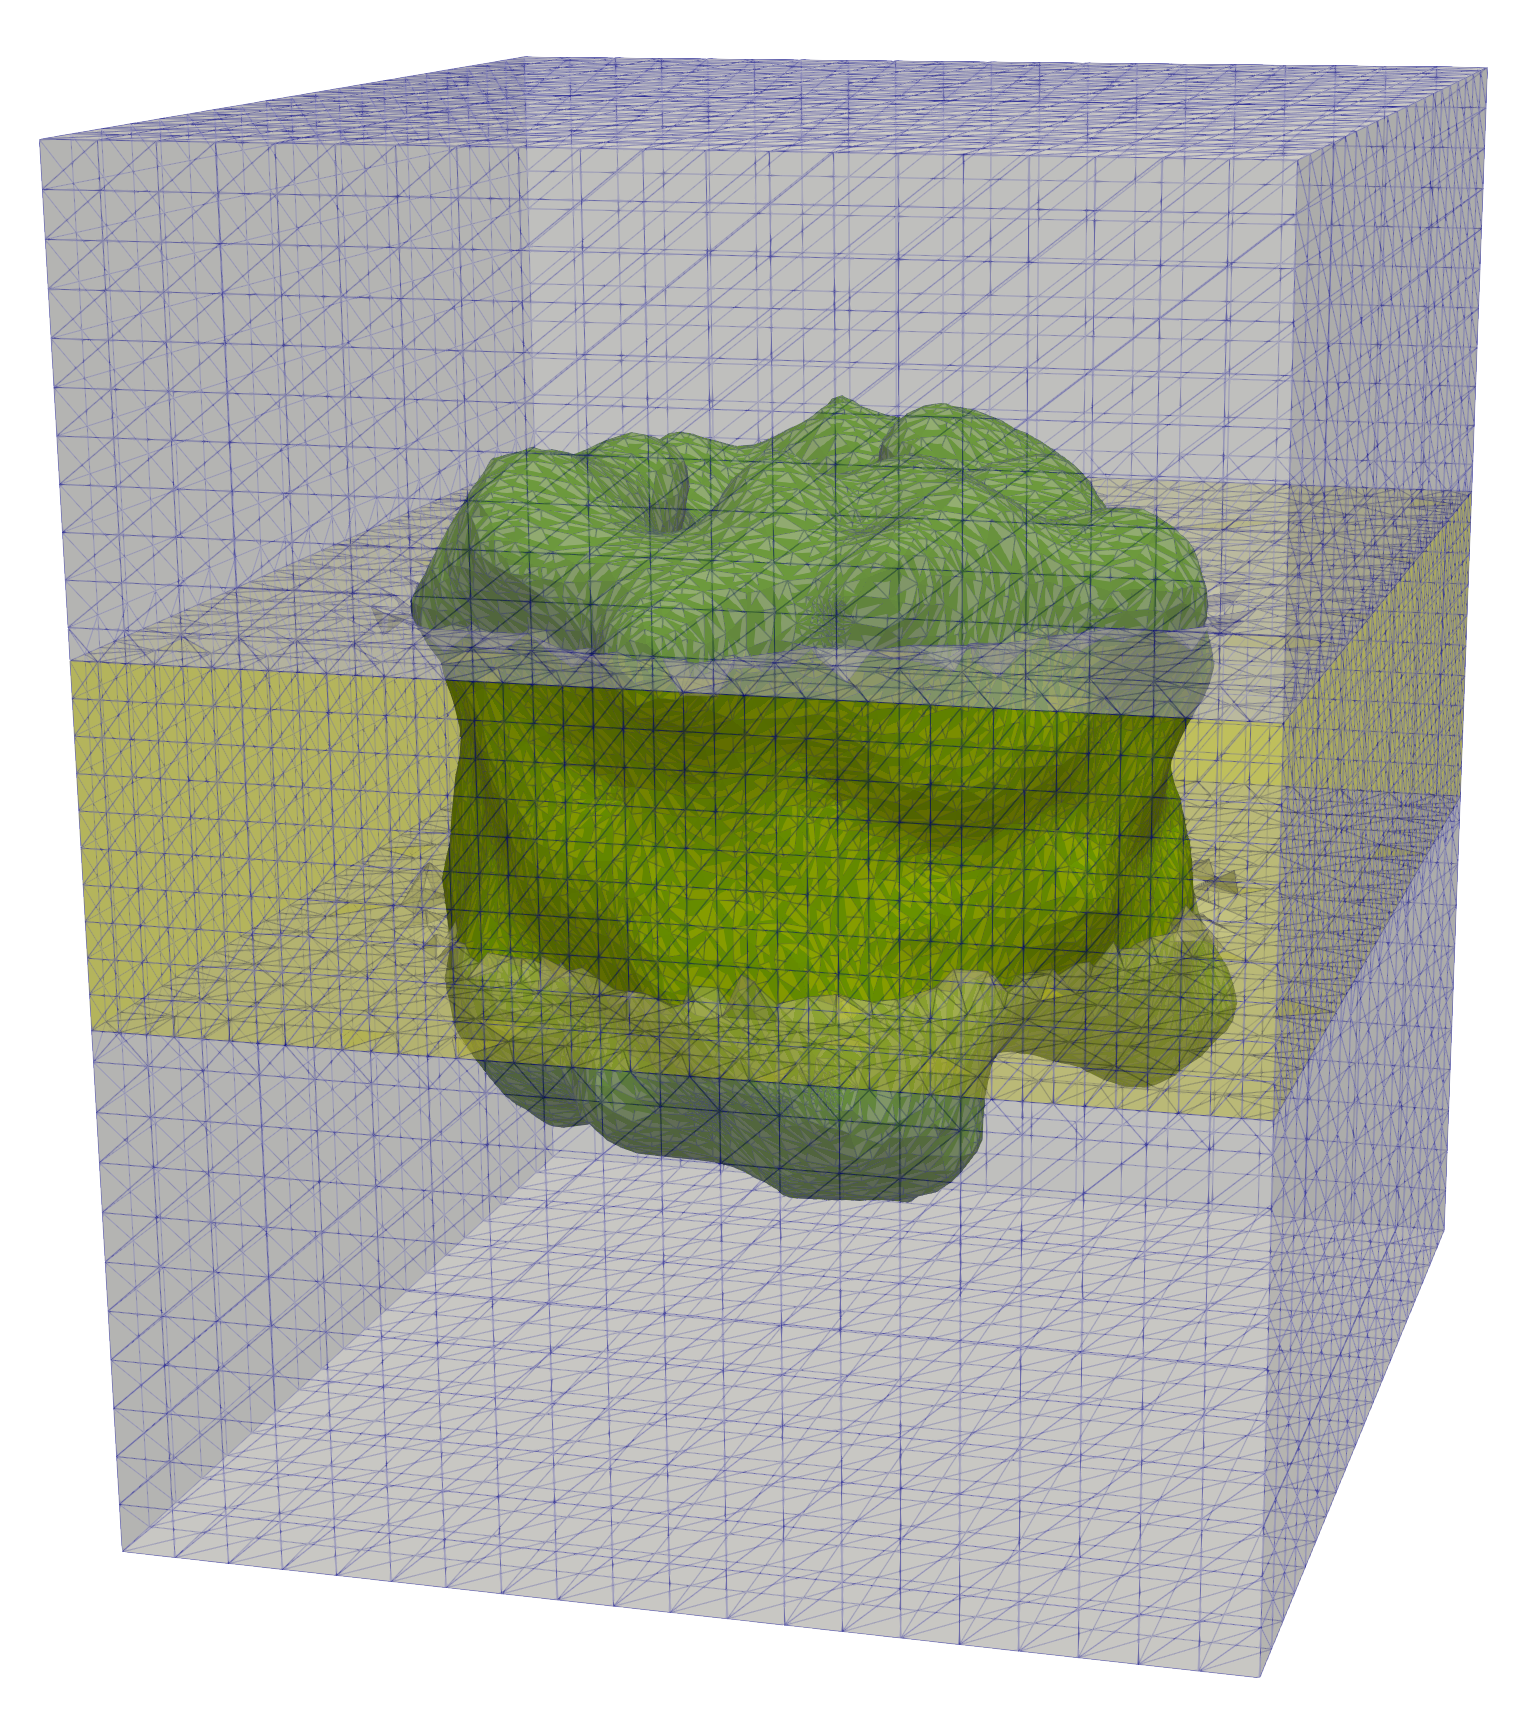
\includegraphics[width=0.8\linewidth]{figures/NewMesh_full_stack.png}
        \caption{Simulation domain mesh}
        \label{fig:omega}
        \end{subfigure}
        \begin{subfigure}[b]{0.49\textwidth}
            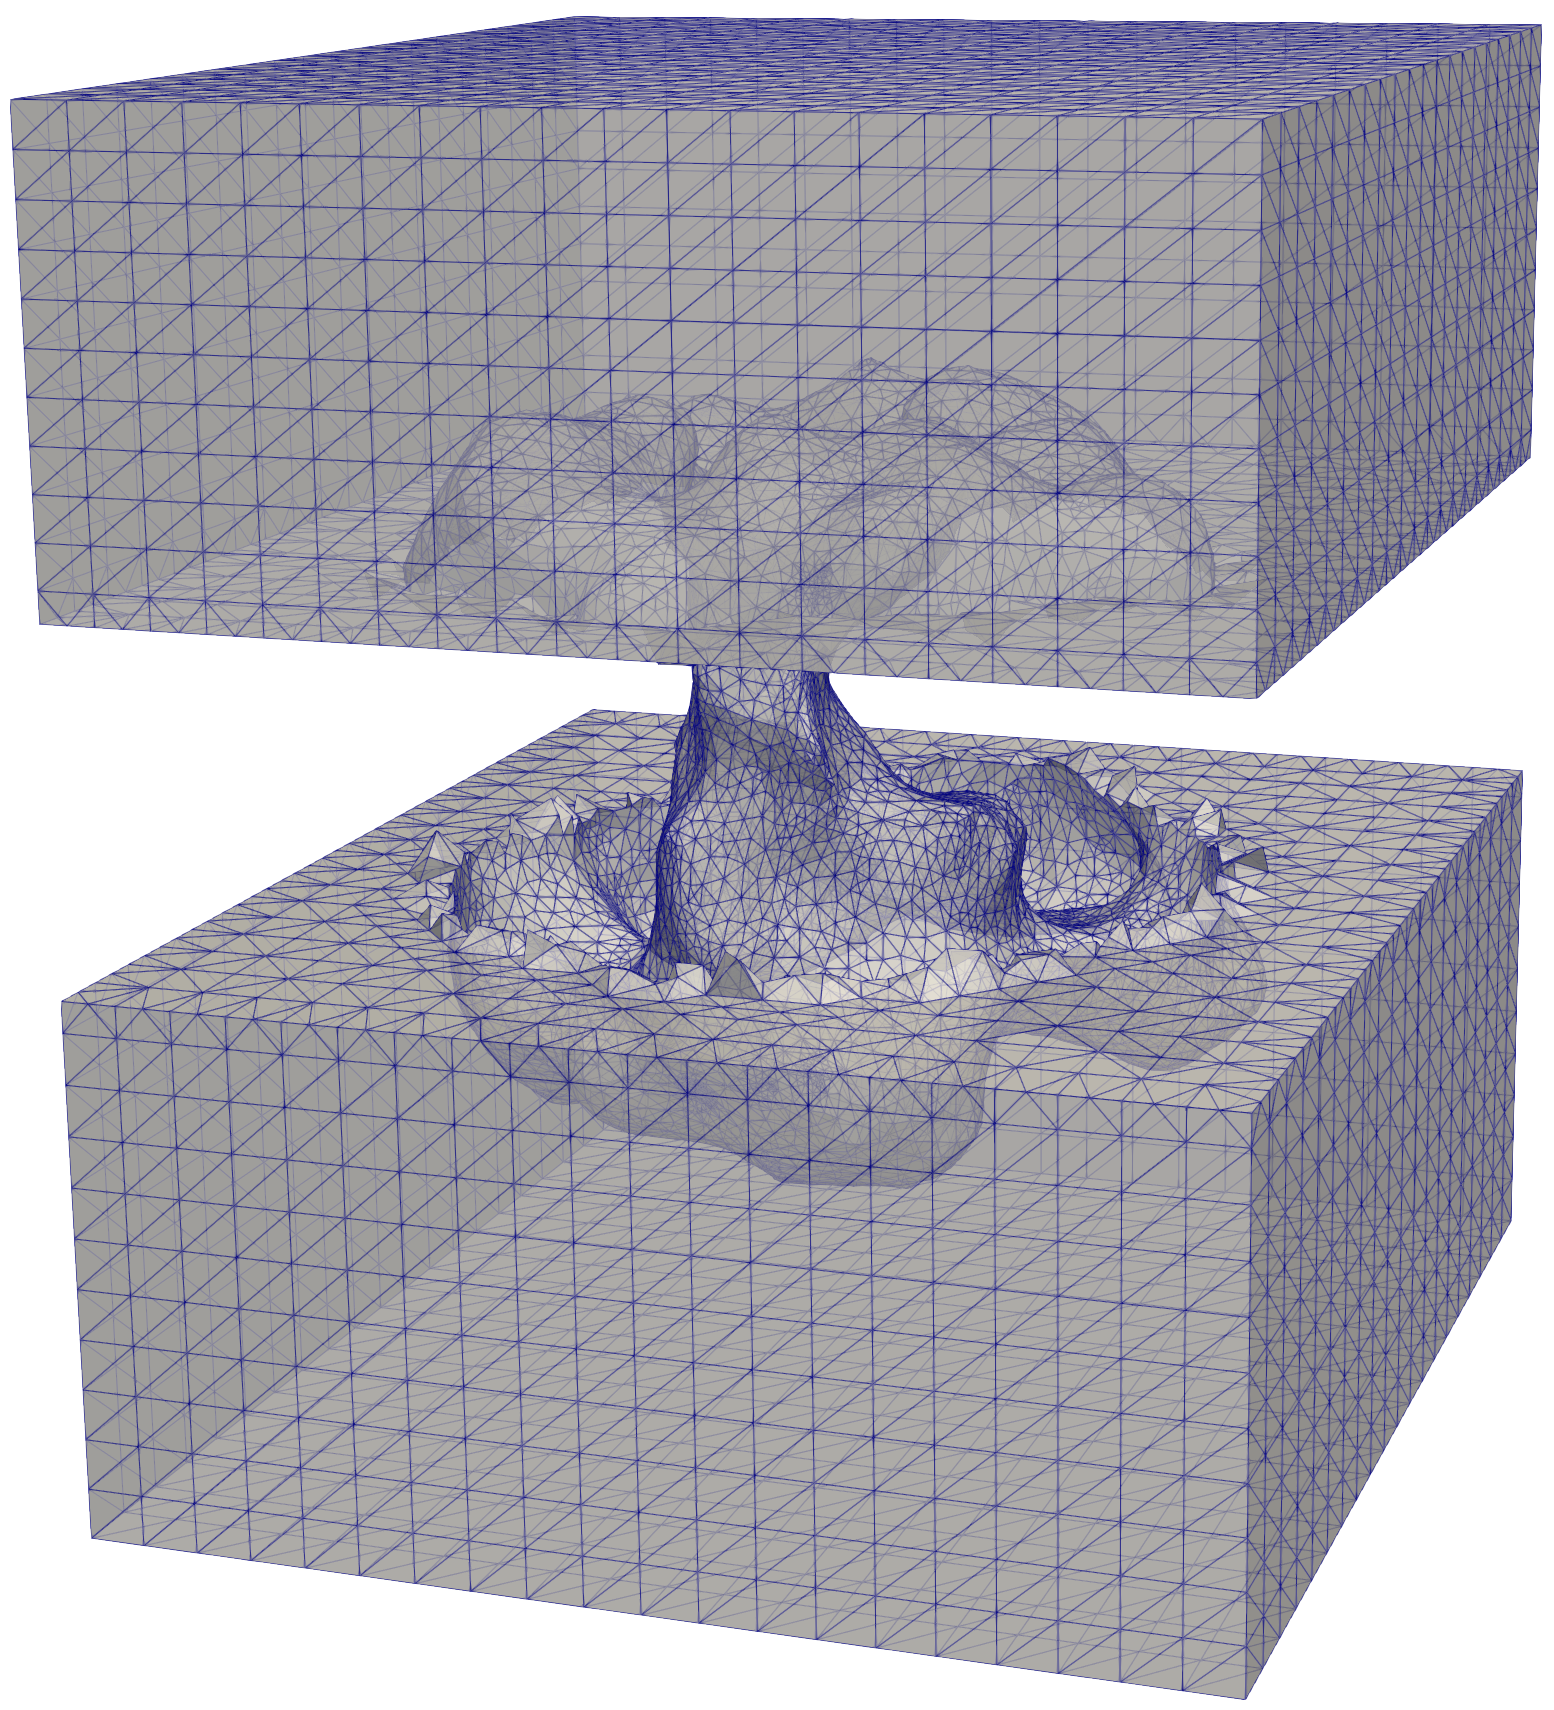
\includegraphics[width=0.8\linewidth]{figures/NewMesh_solvent_only.png}
        \caption{Solvent region mesh}
        \label{fig:Ds}
        \end{subfigure}
    \end{figure}
\end{frame}
\begin{frame}{Applications}
    Numerical solutions to the nonlocal ion channel model can be used in a variety of applications. We are particularly interested in calculating solvation free energies, which are important determinants of VDAC interaction in cellular environments. We have already done some studies of VDAC solvation energies using local models, which we plan to continue. 
\end{frame}
\end{document}
